\documentclass[10pt,a4paper]{article}
\usepackage[utf8]{inputenc}
\usepackage{amsmath}
\usepackage{amsthm}
\usepackage{amssymb}
\usepackage{amsfonts}
\usepackage{amssymb}
\usepackage{mathrsfs}
\usepackage{mathtools}
\usepackage{graphicx}
\usepackage{geometry}
\usepackage{framed}
\usepackage{enumitem}
\usepackage{tabto}
\usepackage{xcolor}
\usepackage{tikz}
\usepackage{tkz-euclide}
\usetikzlibrary{arrows}
\usetikzlibrary{calc}

\usetkzobj{angles}





\newtheorem{theorem}{\color{red}{Teorema}}[section]
\newtheorem{lemma}[theorem]{\color{purple!70}{Lema}}
\newtheorem{proposition}[theorem]{\color{purple!70}{Proposição}}
\newtheorem{conjecture}[theorem]{\color{purple!70}{Conjectura}}
\newtheorem{corollary}[theorem]{\color{purple!70}{Corolário}}
\newtheorem{definition}[theorem]{\color{blue!90}{Definição}}

\newtheorem{remark}[theorem]{\color[rgb]{0,.5,0}{Observação}}
\newtheorem{attention}[theorem]{\color[rgb]{.75,0,0}{Atenção}}

\renewcommand*{\proofname}{Demonstração}

\newcommand{\bref}[1]{\textsuperscript{\tiny\textnormal{\textbf{\setlength{\fboxsep}{1pt}\colorbox{gray!50}{\color{white}{#1}}}}}}

%\endinput



\geometry{
	a4paper,
	total={210mm,297mm},
	left=20mm,
	right=20mm,
	top=15mm,
	bottom=15mm,
}

\setlist[description]{leftmargin=\parindent,labelindent=\parindent,topsep=0pt,itemsep=-1ex,partopsep=1ex,parsep=1ex}
\setlist[itemize]{leftmargin=\parindent,labelindent=\parindent,topsep=0pt,itemsep=-1ex,partopsep=1ex,parsep=1ex}

\author{Gino Chen Hsiang-Jan}
\title{Resumo Álgebra Linear}
\date{26 de Outubro de 2015}

\begin{document}
\maketitle
\tableofcontents

\newpage

%******************************************************************************
% Projeção ortogonal
%******************************************************************************
\section{Projeção ortogonal}
\begin{definition}\bref{[Anton,AlgLinApl-pt,2010]}
Dizemos que dois vetores não nulos $u$ e $v$ em $\mathbb{R}^n$ são ortogonais (ou perpendiculares) se $u.v = 0$. Também convencionamos que o vetor nulo em $\mathbb{R}^n$ é ortogonal a cada vetor em $\mathbb{R}^n$. Um conjunto não vazio de vetores em $\mathbb{R}^n$ é denominado ortogonal se dois quaisquer de seus vetores forem ortogonais. Um conjunto ortogonal de vetores unitários é dito ortonormal.
\end{definition}

\begin{theorem}\bref{[Anton,AlgLinApl-pt,2010]}\\

(a) Se $a$ e $b$ constantes não ambas nulas, então uma equação da forma:\\
\[
	a x + b y + c = 0
\]
representa uma reta em $\mathbb{R}^2$ de normal $n = (a, b)$.\\

(b) Se $a$, $b$ e $c$ constantes não ambas nulas, então uma equação da forma:
\[
	a x + b y + c z + d = 0
\]
representa um plano em $\mathbb{R}^3$ de normal $n = (a, b, c)$.
\end{theorem}

\begin{theorem}\bref{[Anton,AlgLinApl-pt,2010]} \textbf{Teorema das projeções} Se $u, v \in \mathbb{R}^n$ e se $v \neq 0$, então $u$ pode ser escrito de maneira única na forma $u = w_1 + w_2$, em que $w_1$ é um múltiplo escalar de $v$ e $w_2$ é ortogonal a $v$.
\end{theorem}

\begin{definition}\bref{[Anton,AlgLinApl-pt,2010]} No teorema das projeções:\\
	$w_1$ é chamado de projeção ortogonal de $u$ ou componente vetorial de $u$ ao longo de $v$ e denotado como $proj_v u$ e pode ser calculado por: 
	\[
		w_1 = proj_v u = \frac{\langle u, v \rangle}{\langle v, v \rangle} v
	\]
	$w_2$ é chamado de componente vetorial de $u$ a $v$ e póde ser calculado por:
	\[
		w_2 = u - proj_v u = u - \frac{\langle u, v \rangle}{\langle v, v \rangle} v
	\]
\end{definition}
Projeção ortogonal de um ponto em uma reta.
Seja $\mathsf{V} = \mathbb{R}^2$ um espaço vetorial euclidiano, um plano. Dado uma reta $r$ e um ponto $P = (x_1, y_1)$ Desejamos encontrar um ponto $N = (x_0, y_0)$ que é projeção do ponto $P$ na reta $r$. Um ponto $N$ em $r$ que tem a menor distância entre a reta $r$ e o ponto $P$.\\

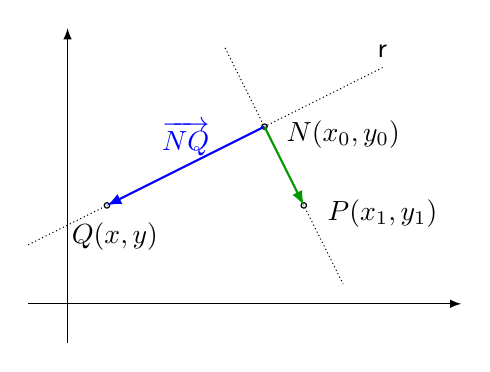
\begin{tikzpicture}[dot/.style={circle,inner sep=1pt,fill,label={#1},name=#1}, line/.style={>=latex}] 
	\coordinate (Q) at ( .5, 1.25) ;
	\coordinate (N) at (2.5, 2.25) ;
	\coordinate (P) at (3.0, 1.25);
	\coordinate (r1)  at (-.5, .75);
	\coordinate (r2) at (4, 3) ;
	\coordinate (s1)  at (2, 3.25);
	\coordinate (s2) at (3.5, 0.25) ;
	\node (QLabel) at ($(Q)+(.1,-.4)$) {$Q(x, y)$};
	\node (NLabel) at ($(N)+(1, -0.1)$) {$N(x_0, y_0)$};
	\node (PLabel) at ($(P)+(1, -0.1)$) {$P(x_1, y_1)$};
	\node (rLabel) at ($(r2)+(0, 0.2)$) {$\mathsf{r}$};
	\draw[->, line] (-.5, 0) -- (5, 0);
	\draw[->, line] (0, -.5) -- (0, 3.5);
	\draw[-, line, densely dotted] ($(r1)$) -- ($(r2)$);
	\draw[-, line, densely dotted] ($(s1)$) -- ($(s2)$);
	\tkzDrawPoints(Q, N, P)
	\draw[->, line, color=blue, thick] ($(N)$) -- node [above] {$\overrightarrow{NQ}$} ($(Q)$);
	\draw[->, line, color=green!60!black, thick] ($(N)$) -- ($(P)$);
	\draw (rLabel);
	\draw (QLabel);
	\draw (NLabel);
	\draw (PLabel);
\end{tikzpicture}

Para de terminar a direção de $r$, vamos escolher um ponto $Q = (x, y)$ em $r$, tal que $\overrightarrow{NQ} = (x - x_0, y - y_0)$ e $Q \neq N$. Então:
\[
	\overrightarrow{NQ} \perp \overrightarrow{NP} \Leftrightarrow \langle(x - x_0, y - y_0), (x_1 - x_0, y_1 - y_0)\rangle = 0
\]
\[
	x_0 ^ 2 - (x + x_1) x_0 + x x_1 + y_0 ^ 2 - (y + y_1) y_0 + y y_1 = 0 \Leftrightarrow
\]

Seja $\mathsf{V}$ um espaço vetorial de corpo $K$ munido de produto interno. $u, v \in \mathsf{V}$, $u \neq 0$ e $v \neq 0$. 

%******************************************************************************
% Transformação Householder
%******************************************************************************
\section{Transformação Householder}
\par
Seja $\mathsf{V}$ um espaço vetorial de corpo $K$ munido de produto interno, $w \in \mathsf{V}$ e $\mathsf{H} \subset \mathsf{V}$ tal que $\mathsf{H}$ é um hiperplano normal a $w$. Deseja-se achar a matriz de transformação $H_w$, onde dado qualquer $x \in \mathsf{V}$ desejamos encontrar um $y \in \mathsf{V}$ tal que $y$ é reflexão de $x$ em relação a $\mathsf{H}$. \\

Para tal finalidade, usaremos uma representação em $\mathbb{R}^2$ para melhor visualizar a dedução.\\

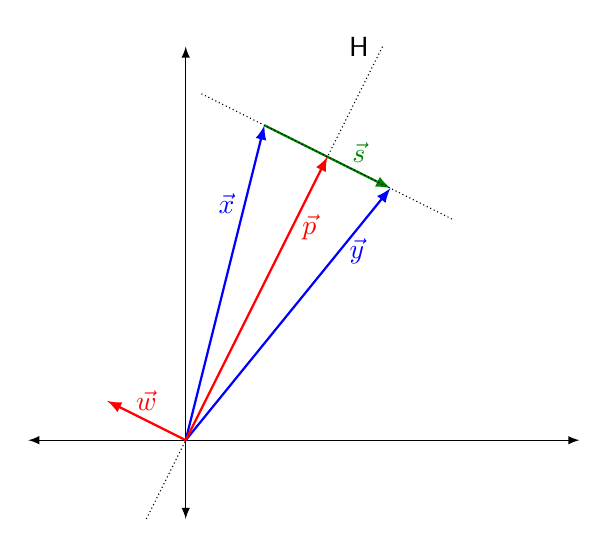
\begin{tikzpicture}[line/.style={>=latex}] 
	\coordinate (w) at (-1, .5);
	\coordinate (wtu) at (1, 2);
	\coordinate (x) at (1, 4);
	\coordinate (wt) at ($2.25/1.25*(wtu)$);
	\coordinate (y) at ($2*(wt)-(x)$);
	\coordinate (V2) at (4, -1);
	\node (HLabel) at (2.2, 5) {$\mathsf{H}$};
	\draw[<->, line] (-2, 0) -- (5, 0);
	\draw[<->, line] (0, -1) -- (0, 5);
	\draw[-, line, densely dotted] (-.5, -1) -- (2.5, 5);
	\draw (HLabel);
	\draw[->, line, color=red, thick] (0, 0) -- node [above] {$\vec{w}$} (w);
	\draw[->, line, color=blue, thick] (0, 0) -- node [left, near end] {$\vec{x}$} (x);
	\draw[->, line, color=blue, thick] (0, 0) -- node [right, near end] {$\vec{y}$} (y);
	\draw[->, line, color=red, thick] (0, 0) -- node [right, near end] {$\vec{p}$} (wt);
	\draw[->, line, color=green!50!black, thick] (x) -- node [above, near end] {$\vec{s}$} (y);
	\draw[-, line, densely dotted] ($2*(x)-(wt)$) -- ($2*(y)-(wt)$);
\end{tikzpicture}
\par
Na figura acima, $p$ como a projeção de $x$ em $\mathsf{H}$ e $s$ é combinação linear de $w$. \\

Projeção de $x$ em $p - x$:\\
\[
	p - x = -\frac{\langle w, x \rangle}{\langle w, w \rangle} w 
\]
\par
temos também:
\[
	s = 2 (p - x) = - 2 \frac{\langle w, x \rangle}{\langle w, w \rangle} w
\]
\par
A reflexão $y$ é $y = x + s$, então:
\[
	y = x - 2 \frac{\langle w, x \rangle}{\langle w, w \rangle} w 
	  = x - 2 \frac{\langle w, x \rangle w }{\langle w, w \rangle}
	  = x - 2 \frac{w \langle w, x \rangle }{\langle w, w \rangle}
\]
\[
	y = x - \frac{2}{w^t w} w.w^t x \Leftrightarrow  
	y = \left(I - \frac{2}{w^t w} w.w^t\right) x
\]
\par
Definimos a transformação linear $H_w$ como:
\[
	H_w(x) = \left(I - \frac{2}{w^t w} w.w^t\right) x
\]

\end{document}

